\section{Results}

\subsection{Performance improved over time and did not differ between groups}

The average accuracy of BCI control increased from \metadataMeanAccuracyFirst~\% in the baseline session to \metadataMeanAccuracyLast~\% in the last session (Fig. \ref{fig:dataset_overview}D). Changes over time were statistically significant ($\beta = \metadataAccuracySessionBeta$, $t(\metadataAccuracySessionDf) = \metadataAccuracySessionTvalue, p \metadataAccuracySessionPvalue, 95\%~\text{CI:}~ [\metadataAccuracySessionBetaCIMin, \metadataAccuracySessionBetaCIMax]$). As shown in the previous analyses of the same dataset \citep{Stieger2020_analysis}, there were no significant differences in the mean accuracy between MBSR (\metadataMeanAccuracyMBSR~\%) and control (\metadataMeanAccuracyControl~\%) groups: $t(\metadataGroupDiffDf) = \metadataGroupDiffTvalue, p \metadataGroupDiffPvalue, \text{Cohen's}~d = \metadataGroupDiffCohensD, 95\% ~\text{CI of the difference}~\allowbreak[\metadataGroupDiffCIMin,  \metadataGroupDiffCIMax]$ (Fig. \ref{fig:dataset_overview}E). The mean accuracy of all participants was \metadataMeanAccuracy\%. At the same time, the intra-individual variability of performance was quite considerable (Fig. \ref{fig:dataset_overview}F). We used linear mixed models to account for this variability in the current analysis.

\subsection{Sensorimotor ROIs contained the majority of task-relevant sources}

For some of the source space analysis pipelines, we identified the task-relevant sources by fitting CSP to distinguish between imaginary movements of two hands. For this purpose, we used EEG during the target presentation interval as it showed a difference in mu power between the imaginary movements primarily over the sensorimotor areas (Fig. \ref{fig:dataset_overview}C). Resulting CSP patterns and the corresponding power spectra for left- and right-hand movements are shown in Fig. \ref{fig:group_csp_source_space_mask}A and Fig. \ref{fig:group_csp_source_space_mask}B, respectively. These patterns were source reconstructed with eLORETA to assess the contribution of individual sources to CSP components (Fig. \ref{fig:group_csp_source_space_mask}C). Sources that exceeded the \cspSourceThreshold th percentile of activity strength were considered task-relevant, and table \ref{supp-tab:csp_sources_per_roi} shows that the sensorimotor ROIs contained the highest number of selected sources. Task-relevant sources formed the resulting source mask (Fig. \ref{fig:group_csp_source_space_mask}D), which was applied to the anatomical definitions of sensorimotor ROIs to obtain a task-based reduced representation (Fig. \ref{fig:pipeline_overview}B).

\begin{figure}[htbp]
    \centering
    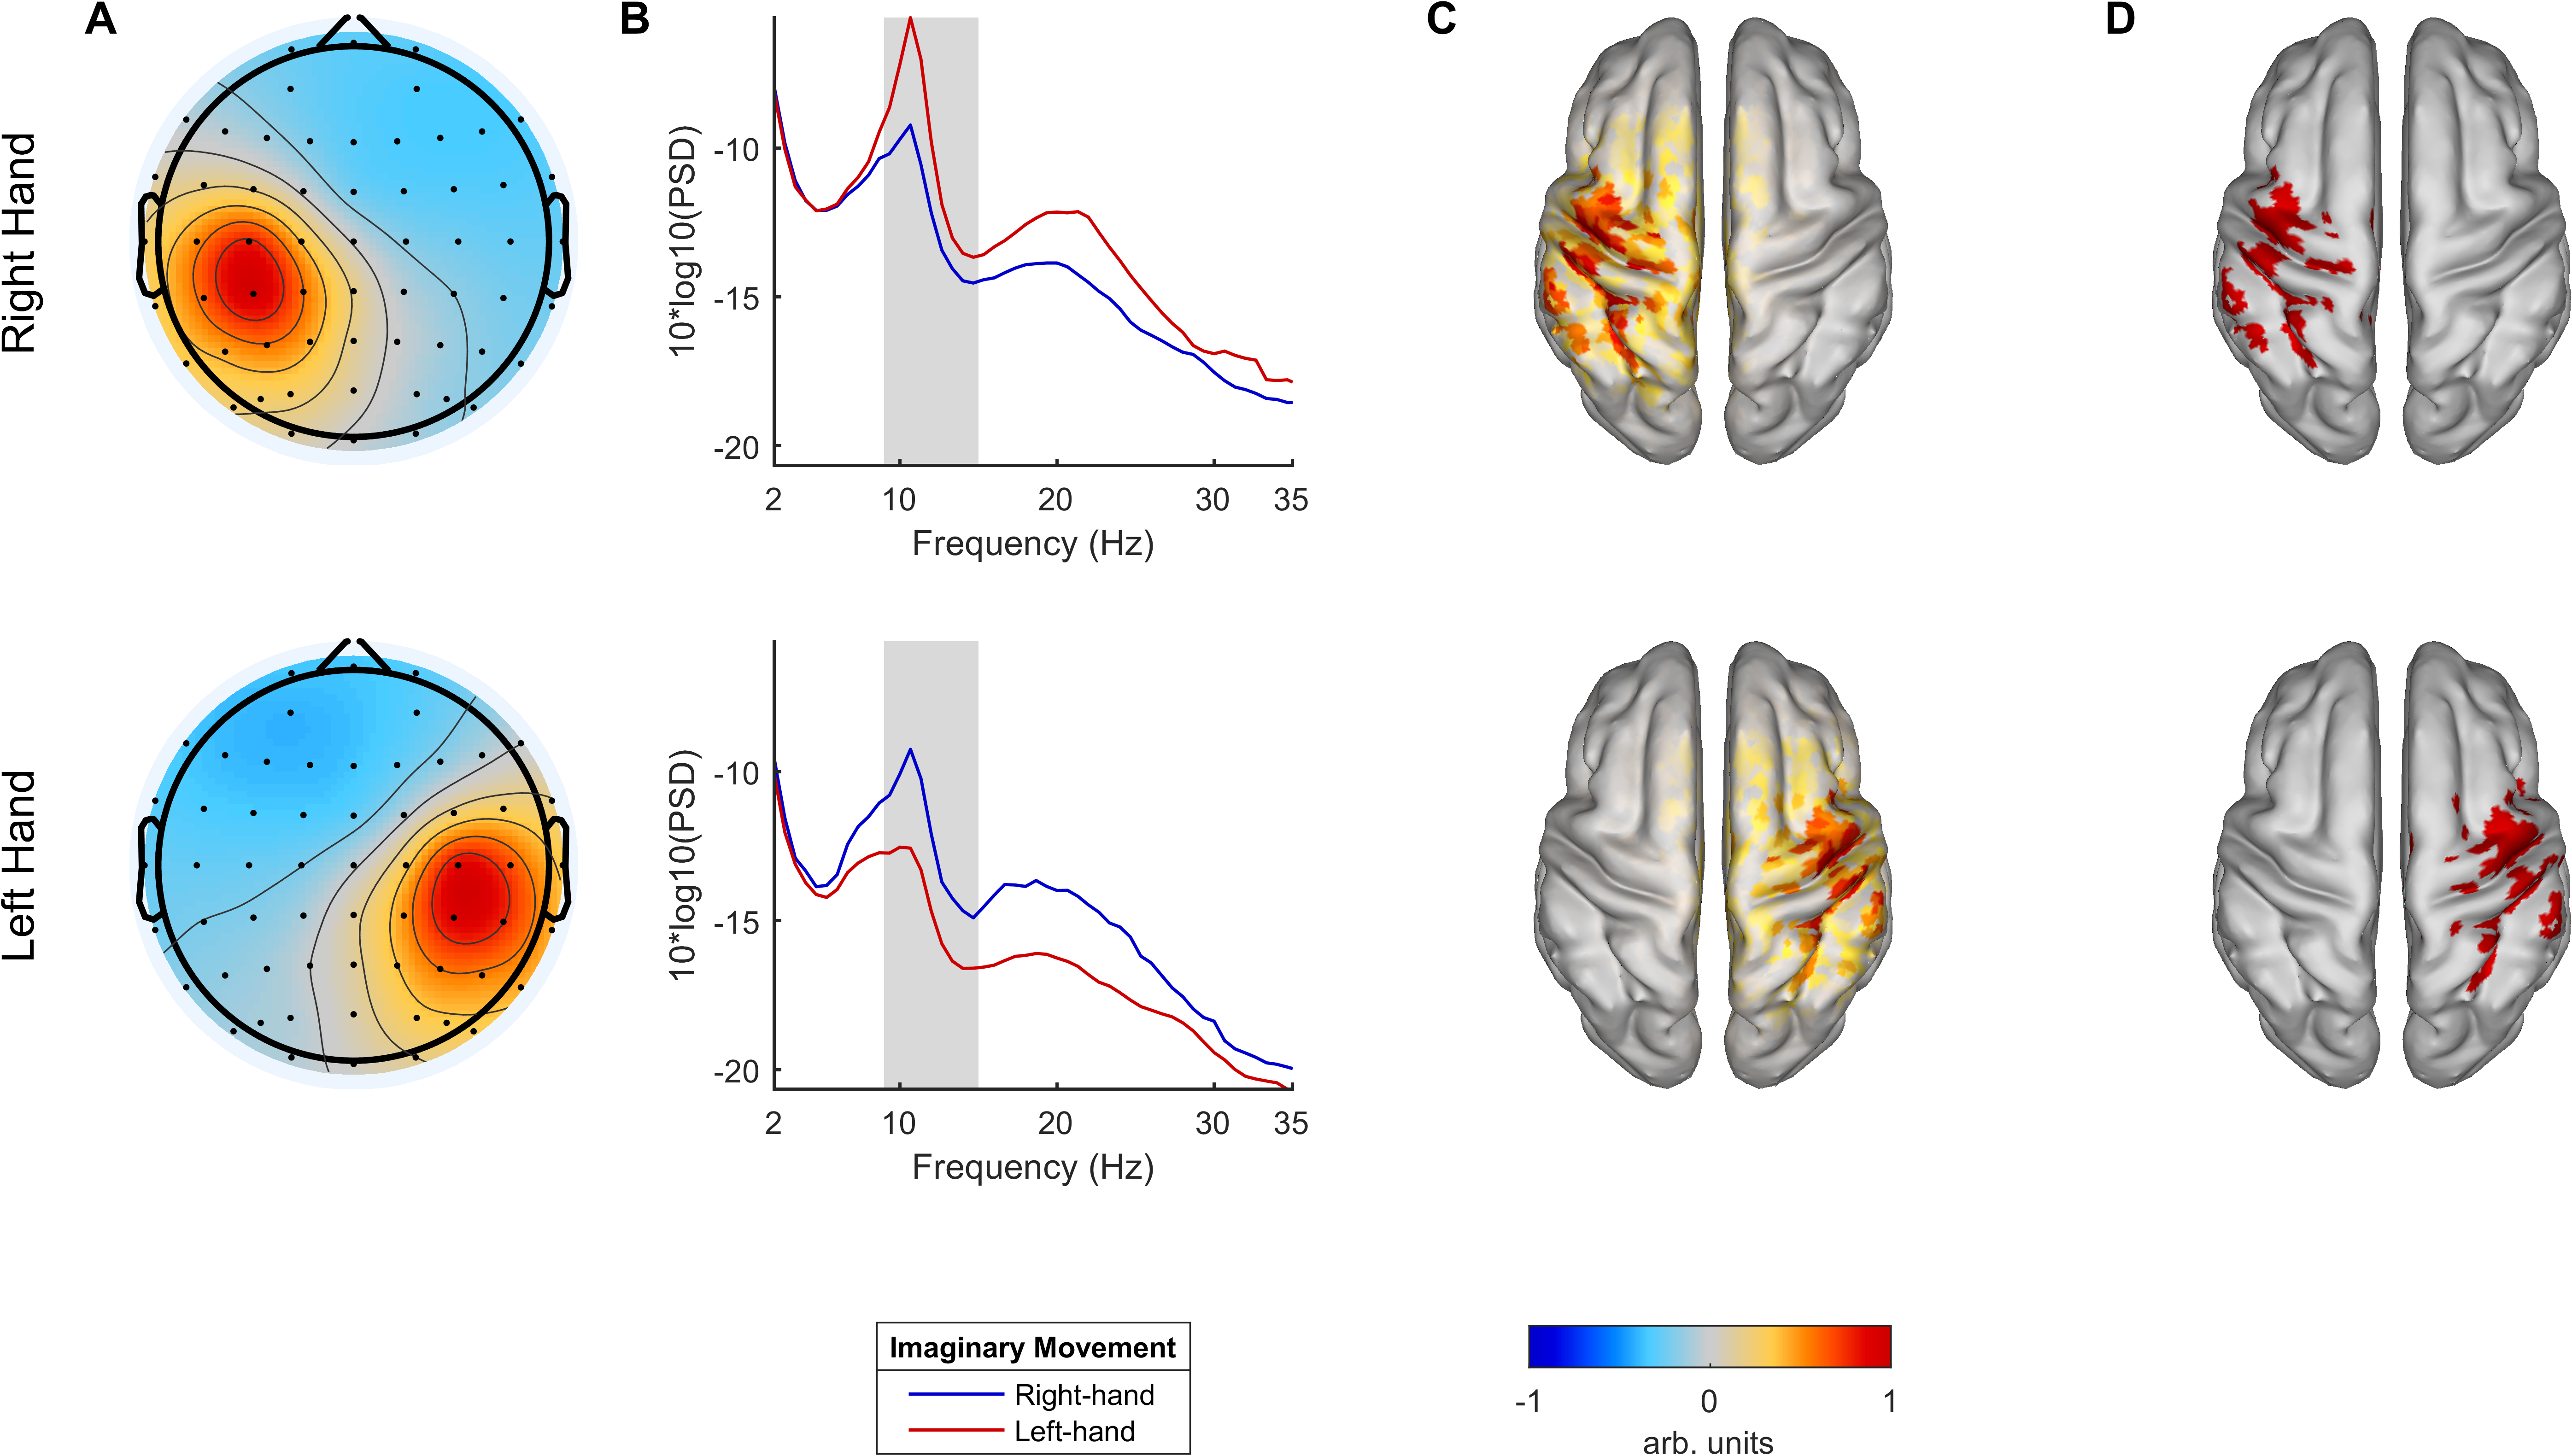
\includegraphics[width=\textwidth]{fig3-group-csp-source-space-mask.png}
    \caption{The task-relevant sources were identified through applying CSP to the EEG data during the target presentation interval after filtering in the \muLow-\muHigh~Hz frequency band. (A) Spatial patterns corresponding to the CSP filters that best discriminate imaginary movements of the right (upper row) and left (lower row) hands. Values were scaled to the [-1, 1] range. (B) Grand average power spectra of the CSP components corresponding to the spatial patterns from (A). The shaded area depicts the \muLow-\muHigh~Hz frequency band that was used to fit CSP. (C) Source reconstruction (absolute values, scaled to [-1, 1] range) of the spatial patterns from (A) with eLORETA. (D) Sources that exceeded the \cspSourceThreshold th percentile of activity strength were considered the most relevant for the execution of the motor imagery task.}
    \label{fig:group_csp_source_space_mask}
\end{figure}

\subsection{Laplace SNR was correlated with BCI performance but did not change over time}

In the sensor space analysis, we used FOOOF to estimate average values of SNR at C3 and C4 after the Laplace transform. Examples of average power spectra for three representative subjects with different levels of Laplace SNR are shown in Fig. \ref{fig:snr_vs_accuracy_session_combined}A. Similar to performance, Laplace SNR did not differ significantly between the participant groups as shown in Fig. \ref{fig:snr_vs_accuracy_session_combined}B ($t(\laplaceGroupDiffSNRDf) = \laplaceGroupDiffSNRTvalue, p \laplaceGroupDiffSNRPvalue, \text{Cohen's}~d = \laplaceGroupDiffSNRCohensD, 95\%~\text{CI of the difference:}~ [\laplaceGroupDiffSNRCIMin, \laplaceGroupDiffSNRCIMax]$). Group-average SNR for different sessions is shown in Fig. \ref{fig:snr_vs_accuracy_session_combined}C.

\medskip

Similar to \citep{Blankertz2010}, we checked whether Laplace SNR was related to successful performance in the BCI training. Subject-average values of Laplace SNR were positively correlated with accuracy ($r=\laplaceSubjectAverageSNRrestAccuracyCor, t(\laplaceSubjectAverageSNRrestAccuracyDf) = \laplaceSubjectAverageSNRrestAccuracyTvalue, p \laplaceSubjectAverageSNRrestAccuracyPvalue, 95\%~\text{CI:}~ [\laplaceSubjectAverageSNRrestAccuracyCIMin, \laplaceSubjectAverageSNRrestAccuracyCIMax]$), showing a between-subject effect of SNR on performance (Fig. \ref{fig:snr_vs_accuracy_session_combined}D). Additionally, the within-subject effect of SNR on accuracy was significant, as assessed with a linear mixed model ($\beta = \laplaceWithinSubjectSNRrestAccuracyBeta, t(\laplaceWithinSubjectSNRrestAccuracyDf) = \laplaceWithinSubjectSNRrestAccuracyTvalue, p \laplaceWithinSubjectSNRrestAccuracyPvalue, 95\%~\text{CI:}~ [\laplaceWithinSubjectSNRrestAccuracyBetaCIMin, \laplaceWithinSubjectSNRrestAccuracyBetaCIMax]$). Figure \ref{fig:snr_vs_accuracy_session_combined}E illustrates the observed within-subject effect.

\medskip

Then, we investigated whether Laplace SNR changed over time due to the training, but longitudinal changes were not significant ($\beta = \laplaceWithinSubjectSNRrestSessionBeta, t(\laplaceWithinSubjectSNRrestSessionDf) = \laplaceWithinSubjectSNRrestSessionTvalue, p \laplaceWithinSubjectSNRrestSessionPvalue, 95\%~\text{CI:}\allowbreak[\laplaceWithinSubjectSNRrestSessionBetaCIMin, \laplaceWithinSubjectSNRrestSessionBetaCIMax]$). Individual and group-level trends are shown in Fig. \ref{fig:snr_vs_accuracy_session_combined}F.

\begin{figure}[htbp]
    \centering
    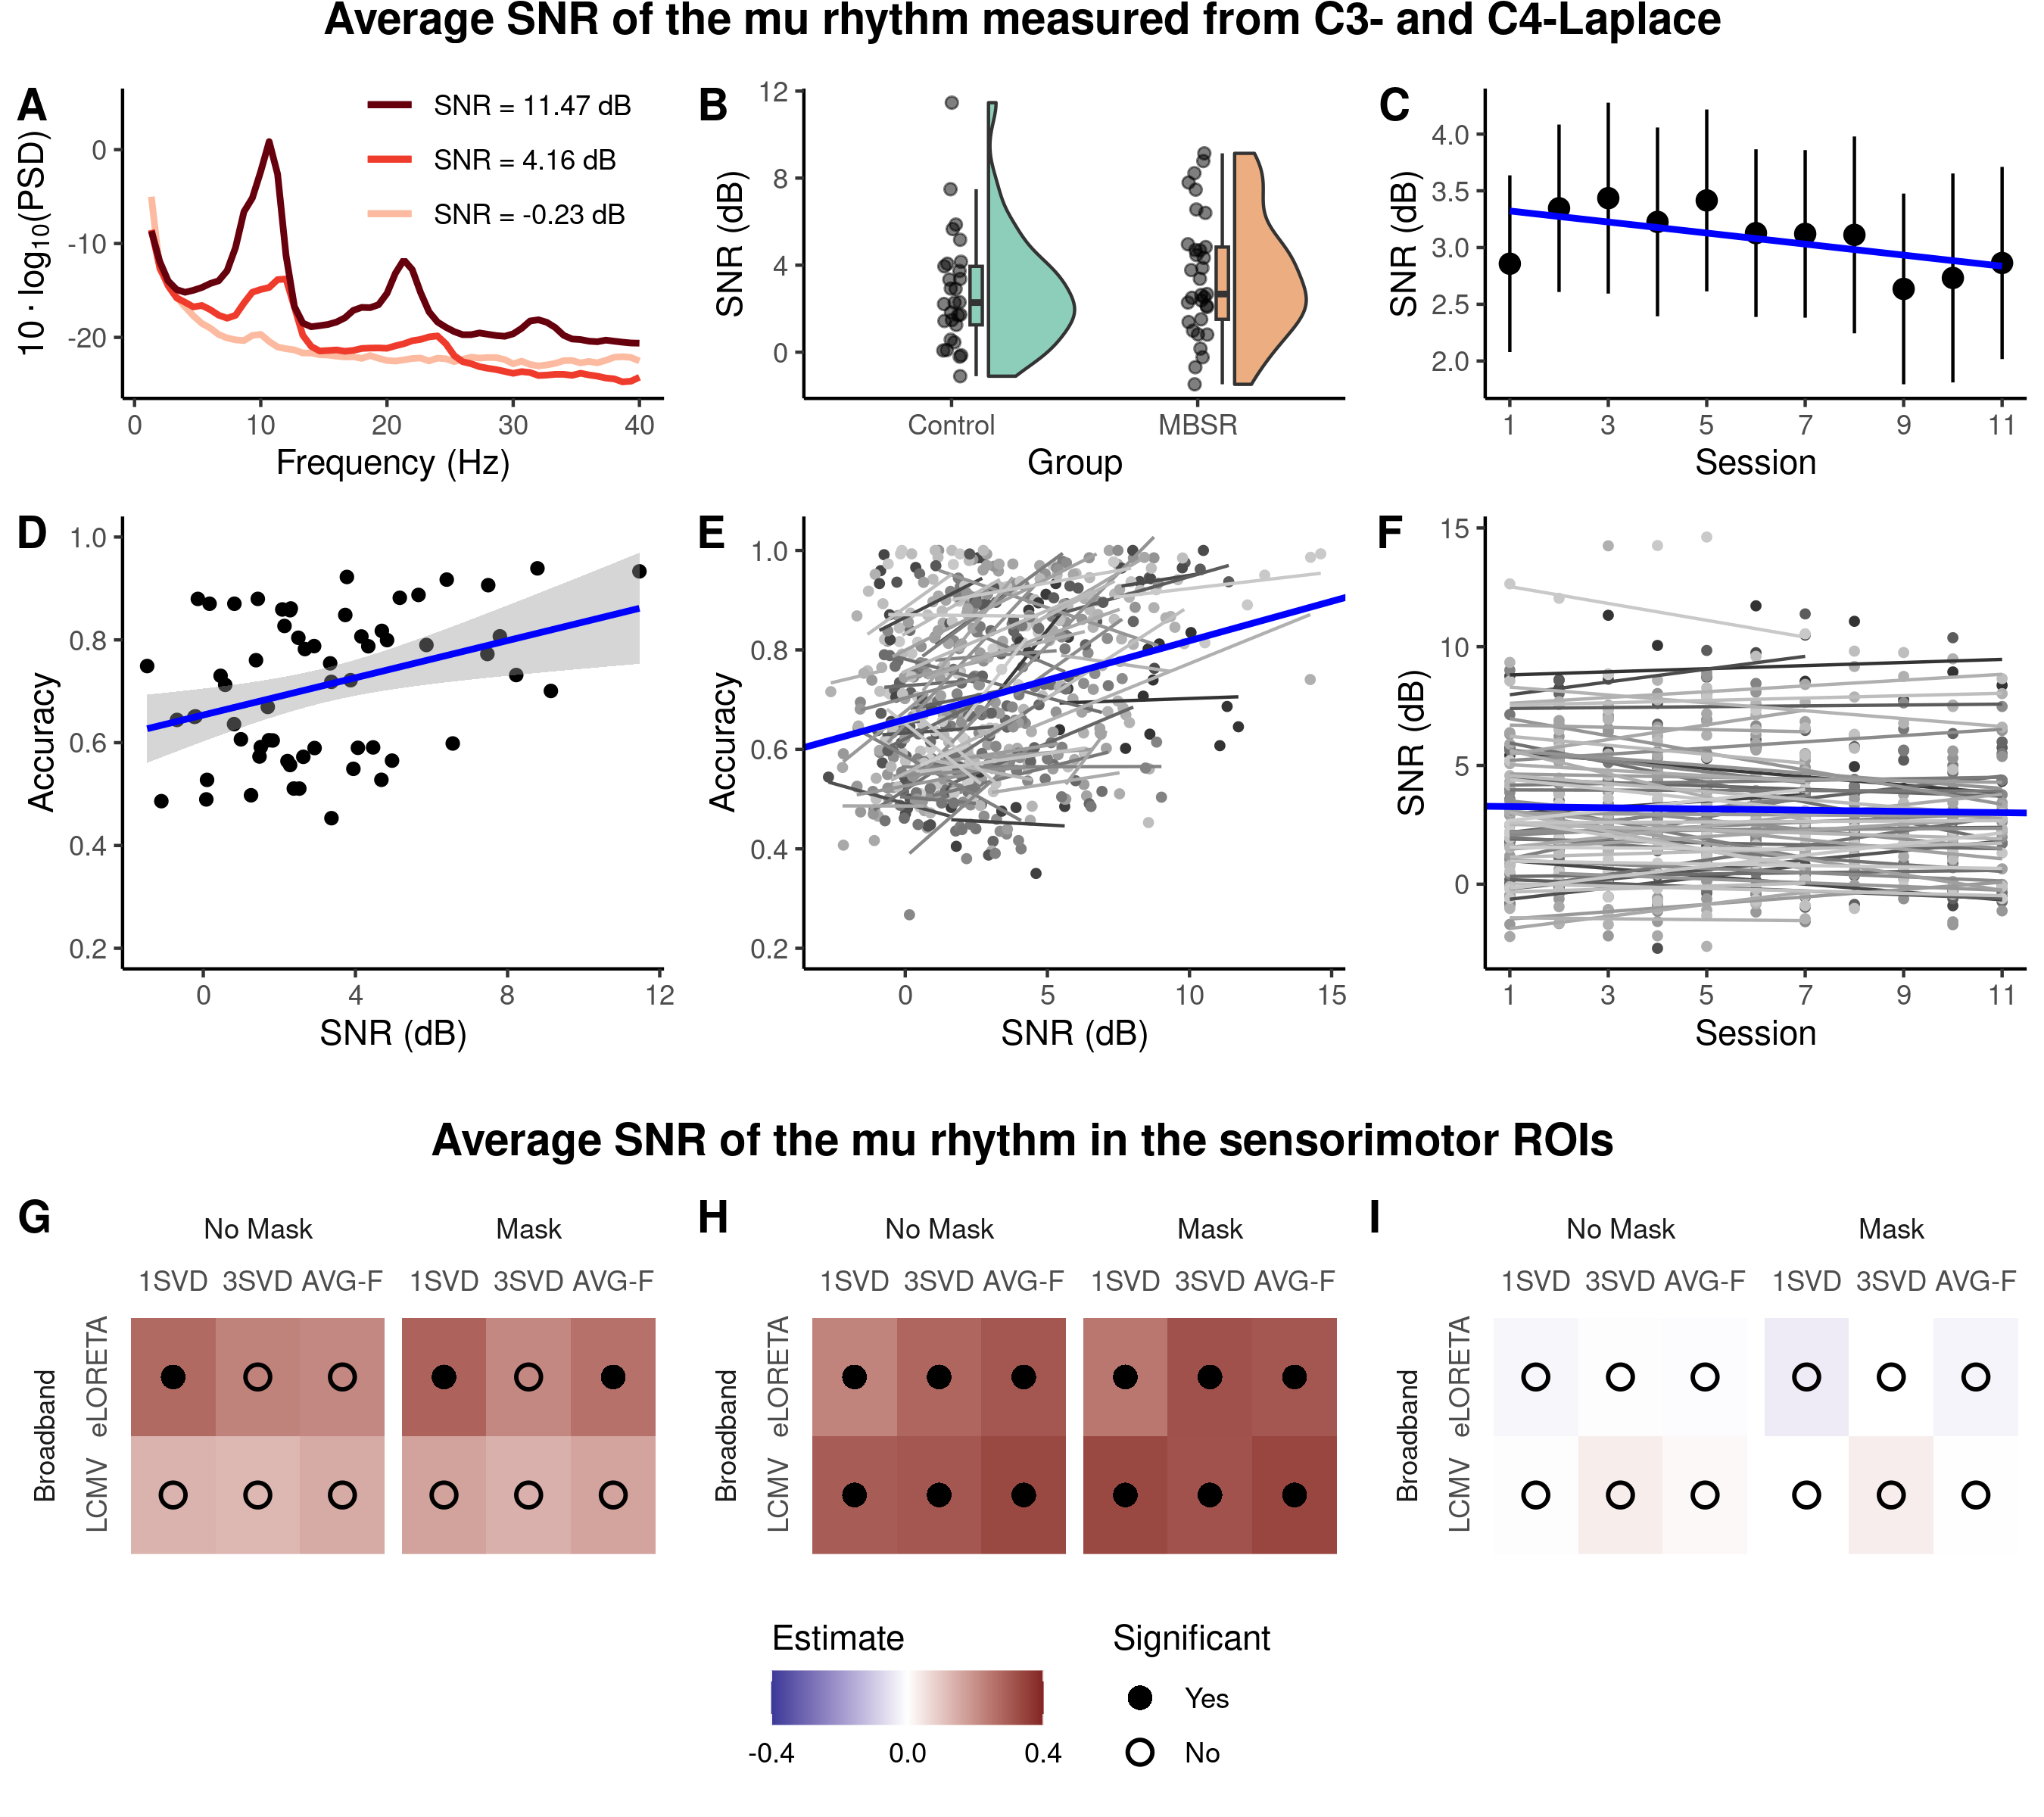
\includegraphics[width=\textwidth]{fig4-snr-rest-accuracy-session.png}
    \caption{Laplace and ROI SNR showed both between- and within-subject effects on BCI performance and did not change systematically throughout the training. (A) Examples of resting-state power spectra (average of C3- and C4-Laplace over all sessions) for representative subjects with different levels of Laplace SNR. (B) The difference in SNR between groups was not significant. (C) Dynamics of group-average SNR across sessions. (D) Accuracy positively correlated with SNR after averaging over all sessions. Each point corresponds to a single participant. (E) Within-subject variability of BCI performance was related to session-to-session changes in SNR. Each point corresponds to a single session. Within-subject (gray) and group-level (blue) linear trends are shown. (F) No longitudinal changes were observed for SNR. Within-subject (gray) and group-level (blue) linear trends are shown. (G-I) Multiverse analysis similar to (D-F) but for ROI SNR in the source space showed high consistency of SNR-related effects across the data processing pipelines.}
    \label{fig:snr_vs_accuracy_session_combined}
\end{figure}

\subsection{Effects of SNR, but not phase synchronization, were stable in the multiverse analysis}

For the ROI SNR and phase synchronization, we applied a multiverse analysis to investigate the robustness of the observed effects to the selection of the pipeline. Figures \ref{fig:snr_vs_accuracy_session_combined}G and \ref{fig:snr_vs_accuracy_session_combined}H show that the estimated effects of ROI SNR on accuracy were positive for all \numBBPipelines~broad-band pipelines both on the between- and within-subject level, respectively. Additionally, on the within-subject level, all effects were significant. Figure \ref{fig:snr_vs_accuracy_session_combined}I shows that no significant longitudinal changes in ROI SNR were observed for all considered pipelines. Overall, the results of the multiverse analysis for ROI SNR corresponded to the results for Laplace SNR and showed that the selection of the pipelines did not affect the observed effect of SNR on performance and changes in SNR.

\medskip

For the phase synchronization, we first checked whether the grand-average spectra of within- and across-hemisphere values of PS measures show a pronounced peak in the mu frequency range. Such a peak indicates that the interaction is specific to the ongoing mu oscillations. As shown in Fig. \ref{fig:snr_connectivity}A for a selection of pipelines, the peak was pronounced in most cases. However, within-hemisphere coherence estimated using the first SVD component showed almost identical values in the whole frequency range. In this case, it might occur due to the volume conduction, which equally affects all the frequencies.

\medskip

In line with the previous studies \citep{Bayraktaroglu2013, Vidaurre2020}, we observed a robust positive effect of SNR on ImCoh and LagCoh, which are not sensitive to both spurious (caused by volume conduction) as well as genuine zero-lag interactions (Fig. \ref{fig:snr_connectivity}B). In contrast, the effects of SNR on coherence were less consistent between pipelines and differed in sign depending on the selection of the processing methods. Overall, these results confirm that it is necessary to correct for SNR in the analyses of effects related to phase synchronization.

\begin{figure}[htbp]
    \centering
    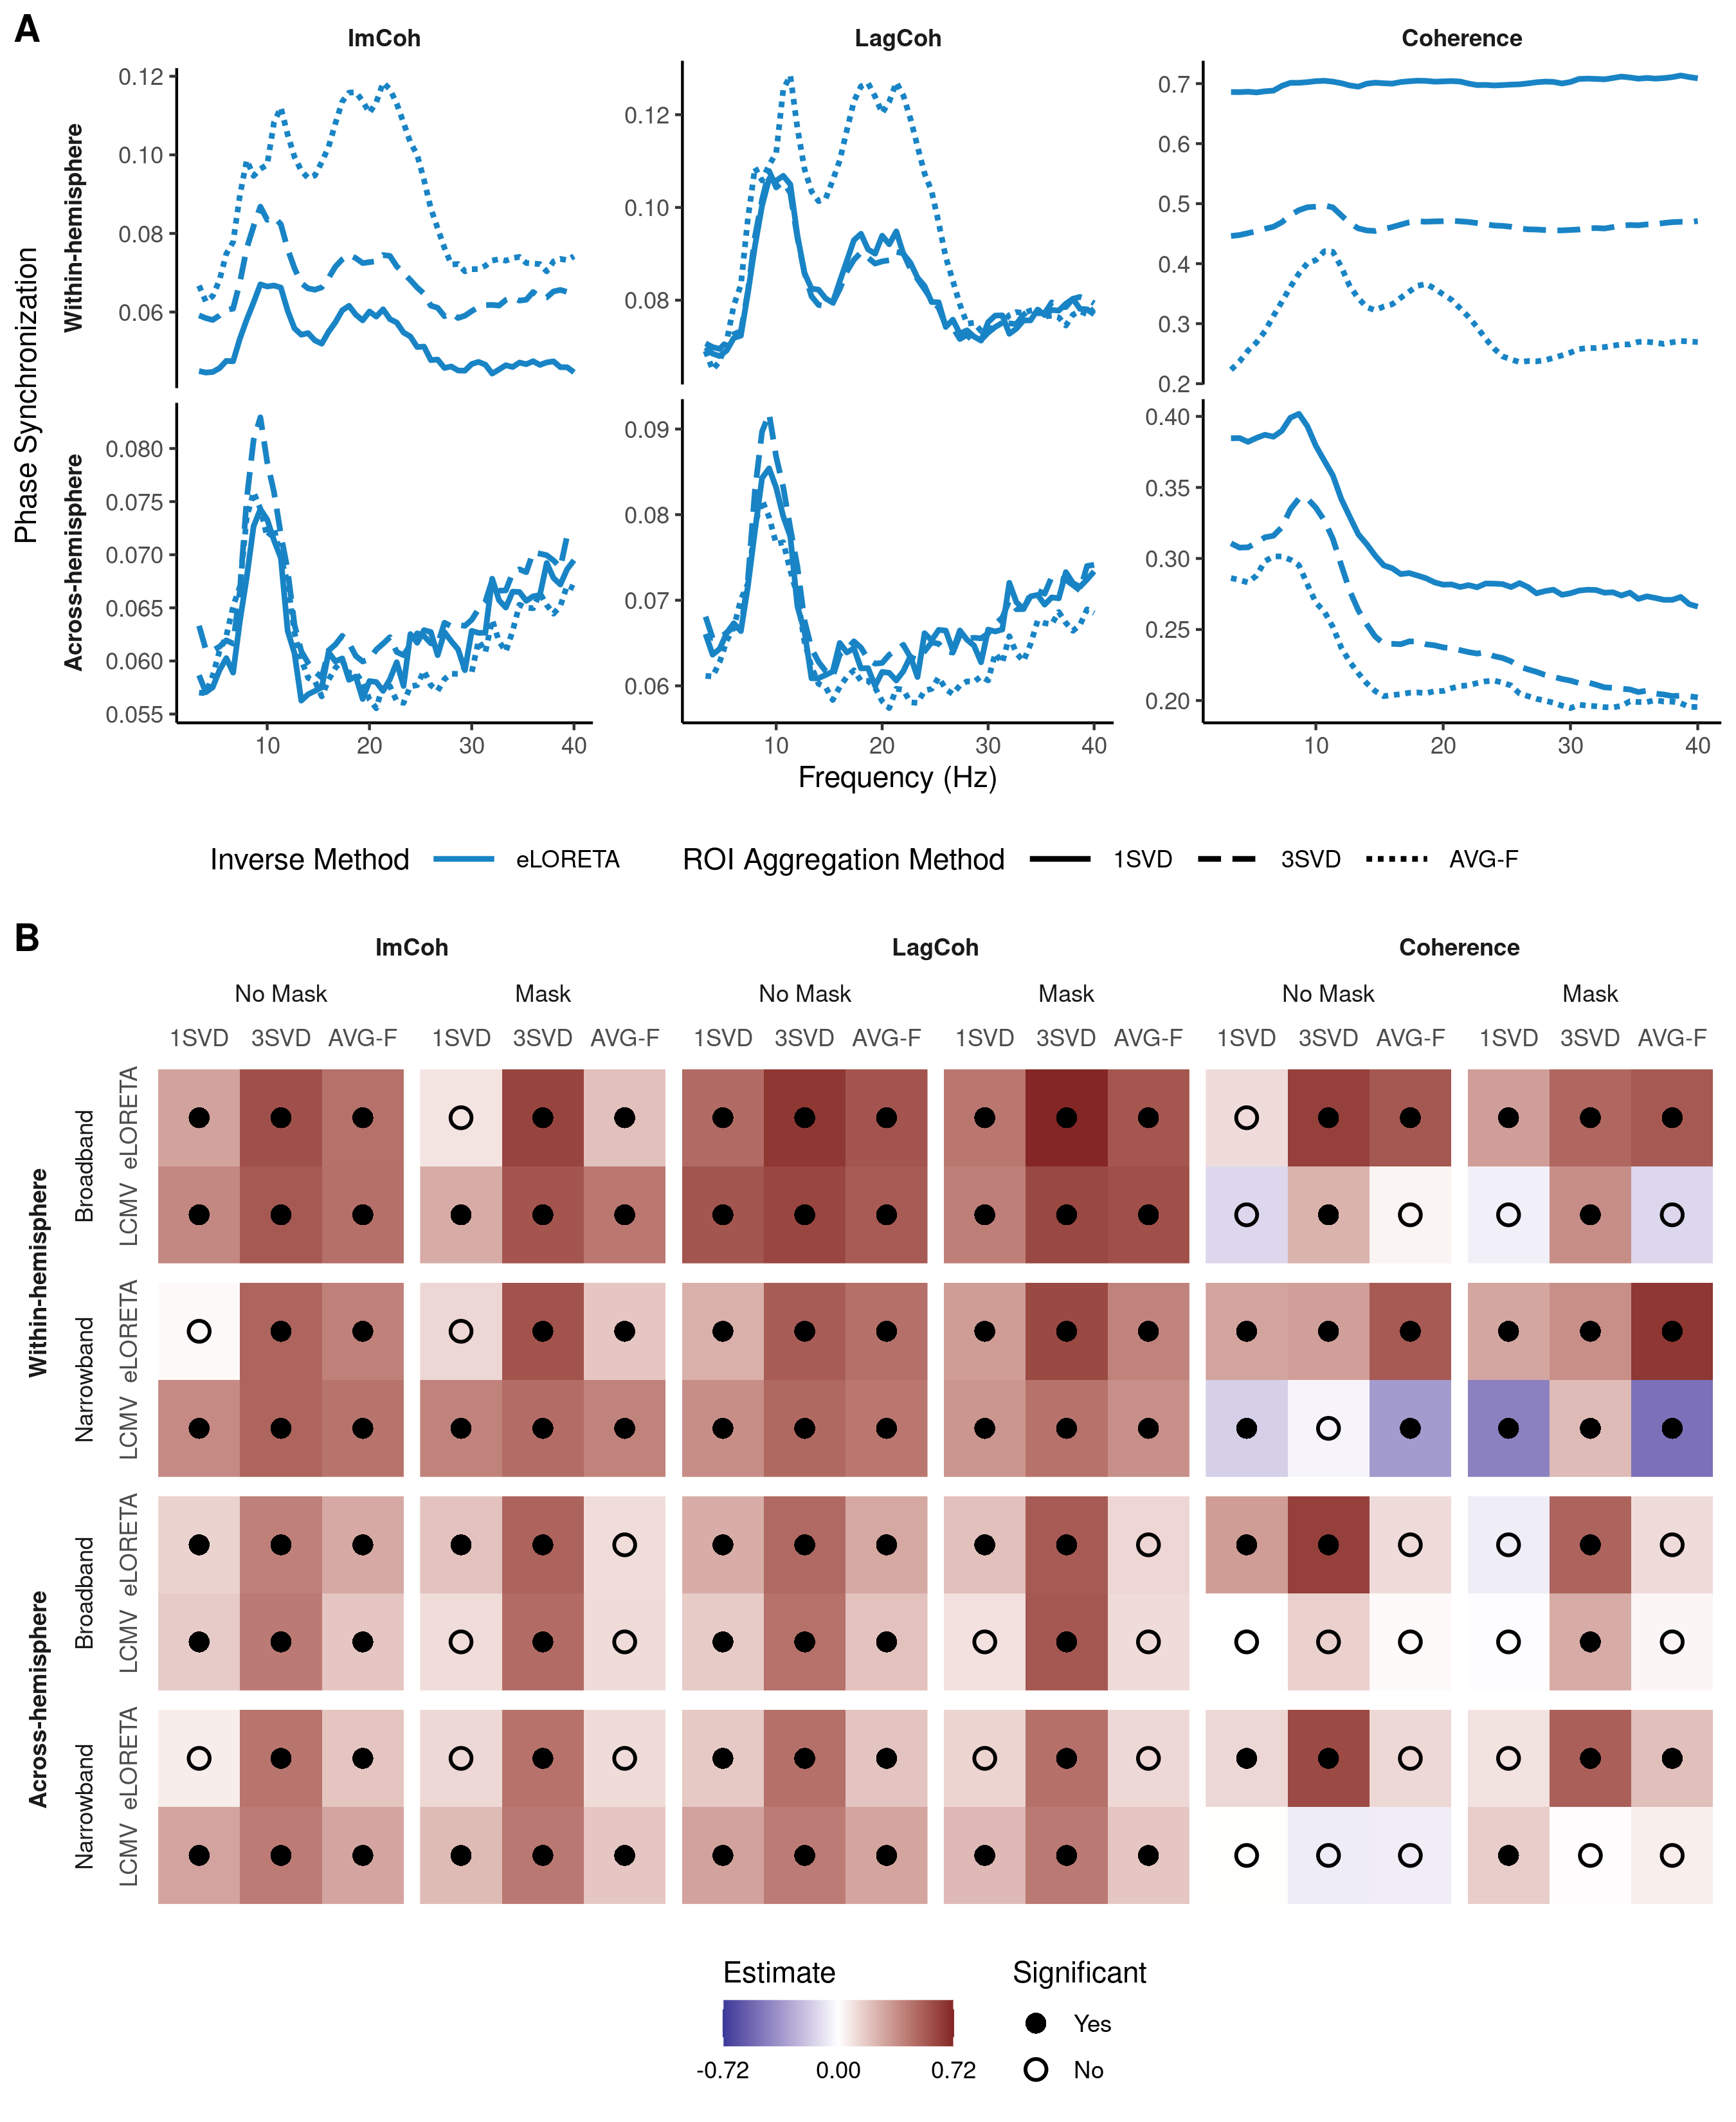
\includegraphics[width=\textwidth]{fig5-snr-connectivity.png}
    \caption{Multiverse analysis of the relationship between SNR and phase synchronization measures. (A) Grand average spectra of within- (top row) and across-hemisphere (bottom row) values of ImCoh, LagCoh, and coherence (columns: left to right) for the broadband pipelines with eLORETA, anatomical definitions of ROIs, and different ROI aggregation methods. (B) SNR showed consistent positive effects on ImCoh and LagCoh but not on coherence, both for within- and across-hemisphere phase synchronization.}
    \label{fig:snr_connectivity}
\end{figure}

\medskip

Then, we investigated the relationship between phase synchronization and accuracy as well as changes in PS over time. For both research questions, effects were not significant for the majority of the pipelines and PS measures (Fig. \ref{fig:multiverse_connectivity_performance_within}). Nevertheless, the pipelines that led to significant results often corresponded to a choice of a particular method at different processing steps. For example, the effects of within-hemisphere ImCoh and LagCoh on accuracy were more likely to be significant when inverse modeling was performed with an LCMV beamformer (Fig. \ref{fig:multiverse_connectivity_performance_within}A, rows 2, 4, and 6 from the top). In this case, pipeline-specific results showed up as stripes in the visualization. A different tendency was observed for the between-subject effect of phase synchronization on accuracy (Fig. \ref{supp-fig:multiverse_connectivity_performance_between}) as well as longitudinal changes in PS (Fig. \ref{supp-fig:multiverse_connectivity_longitude}): When assessing phase synchronization using coherence, significant effects were more likely to emerge than for other PS measures. Overall, the effects of connectivity on performance were not significant for the majority of the pipelines, and the direction of the effects was not consistent between different pipelines and PS measures.

\begin{figure}[htbp]
    \centering
    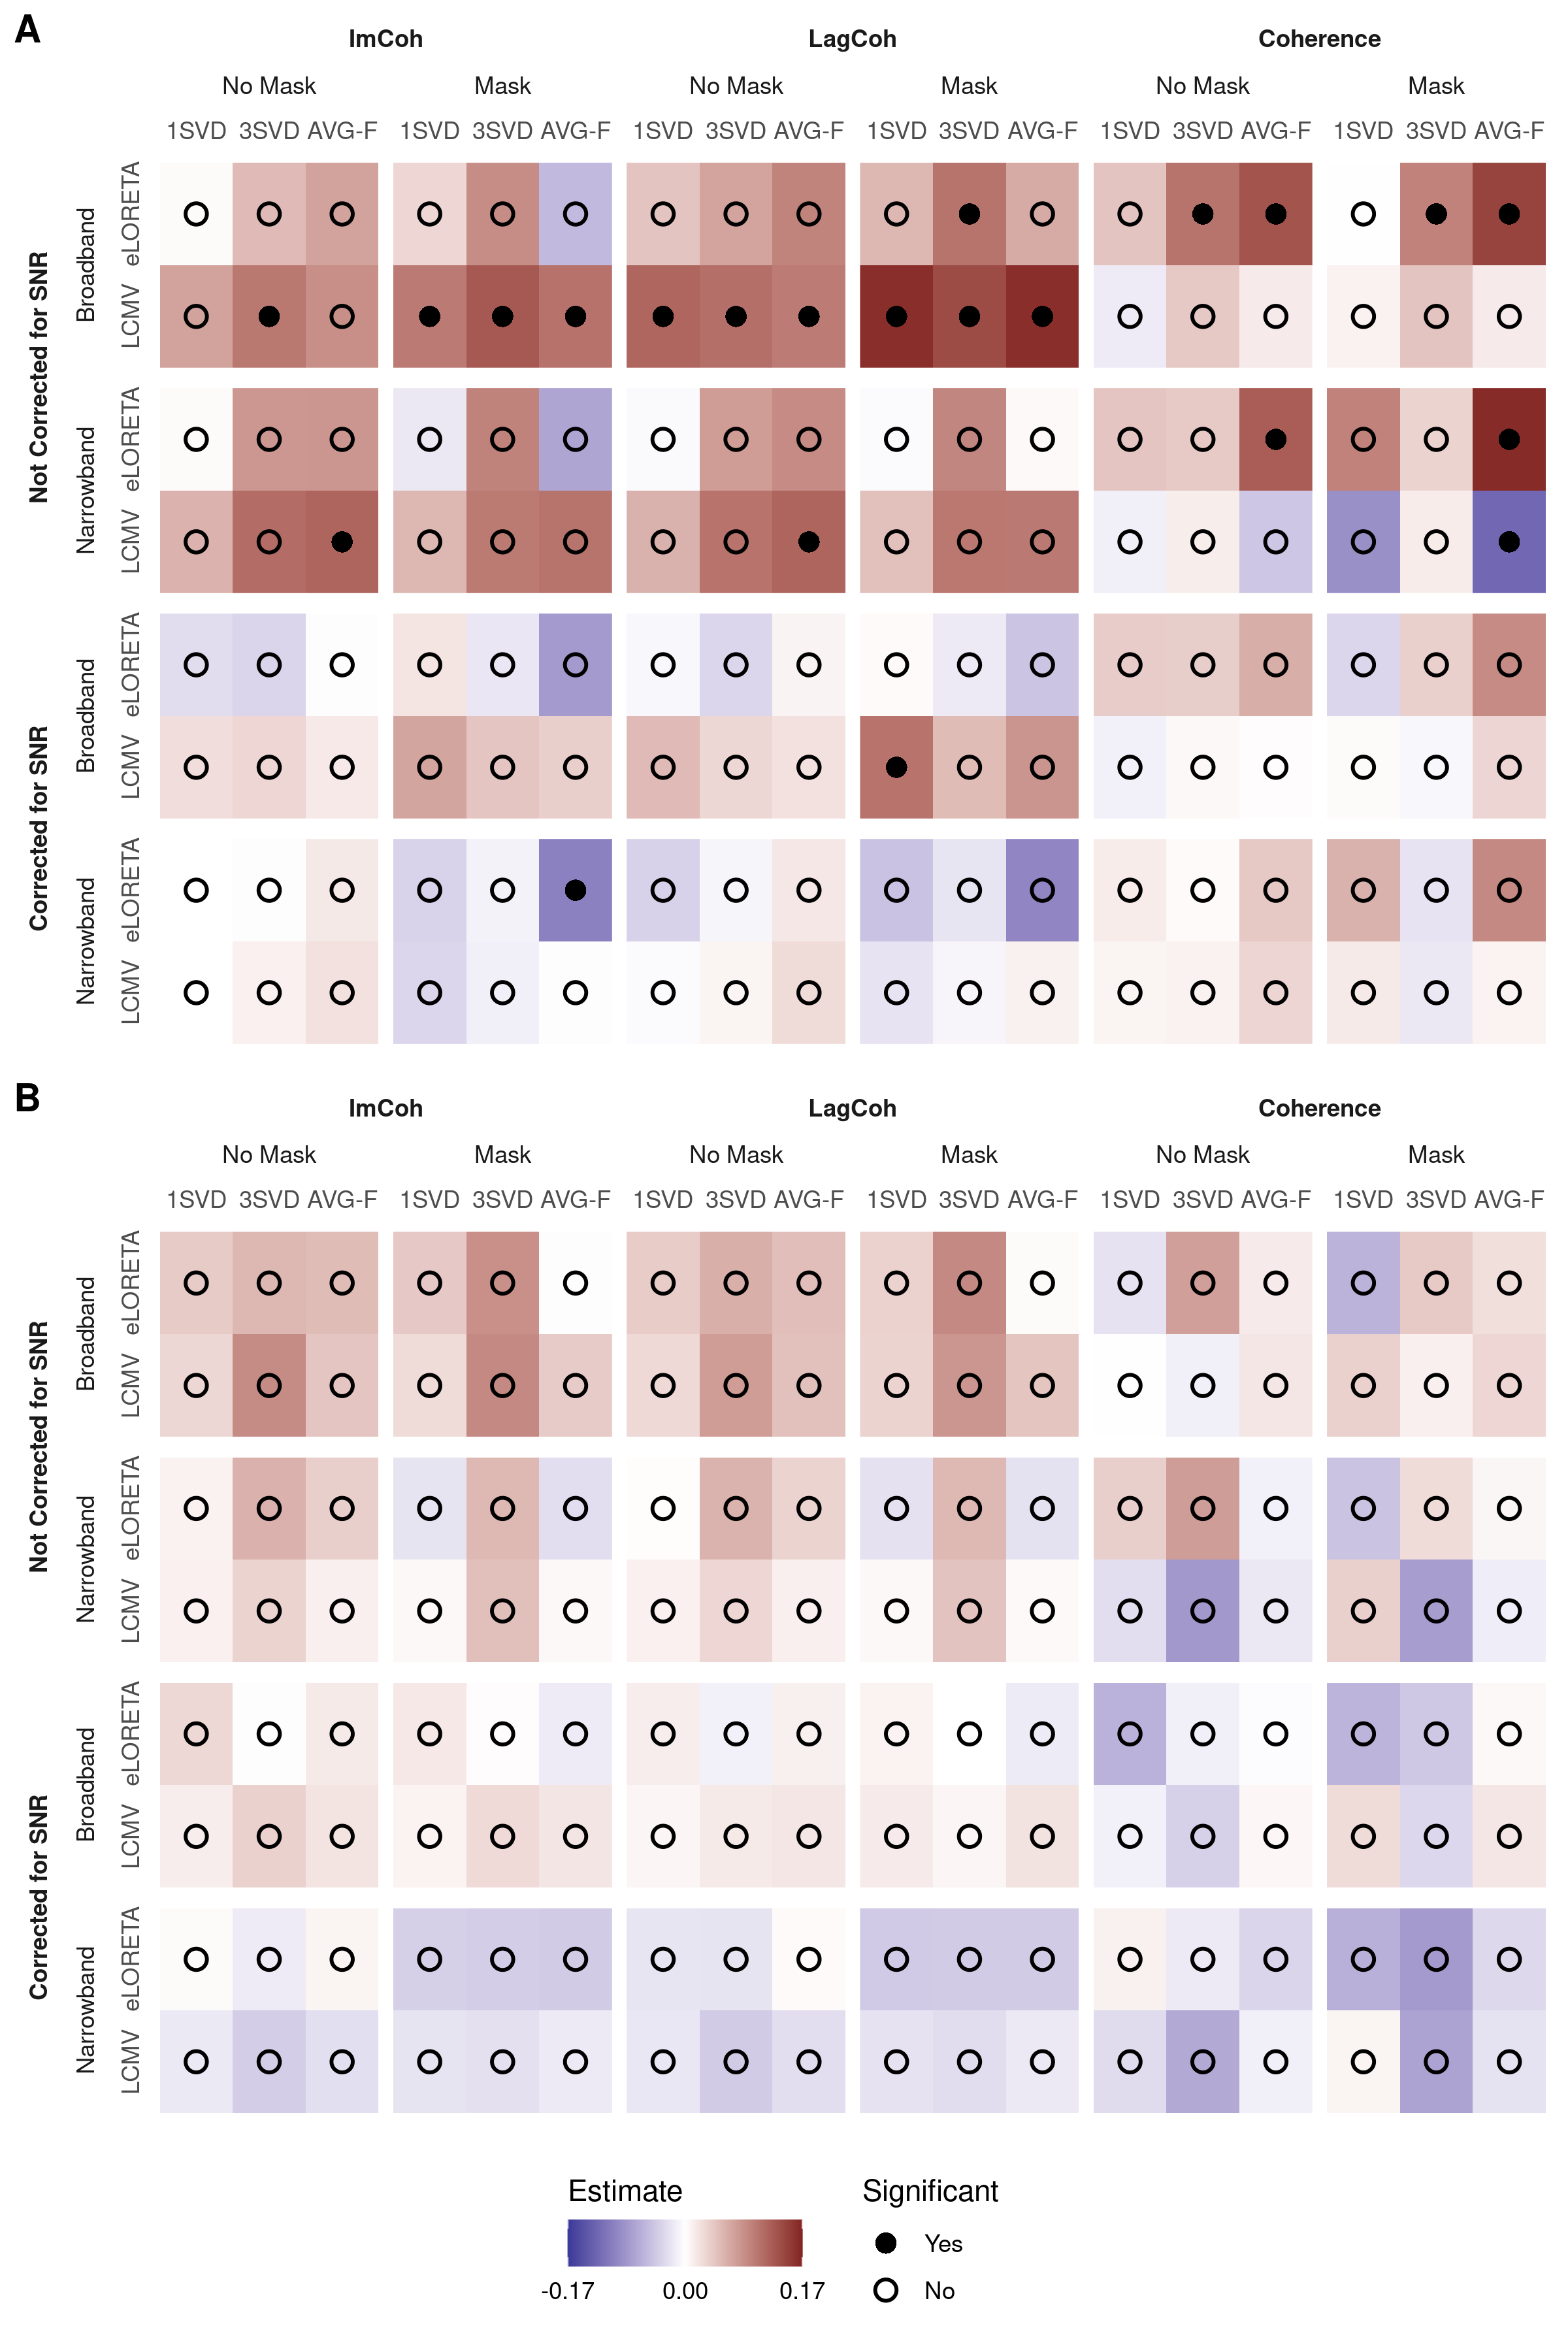
\includegraphics[width=0.95\textwidth]{fig6-multiverse-connectivity-performance-within.png}
    \caption{Within-subject effects of phase synchronization on BCI performance in the split multiverse analysis. Bonferroni correction for multiple ($m = \numComparisons$) comparisons was applied. Panels (A) and (B) correspond to within- and across-hemisphere phase synchronization, respectively.}
    \label{fig:multiverse_connectivity_performance_within}
\end{figure}

\medskip

Finally, we ran a joint analysis for all research questions by pooling together the data from all of the pipelines and fitting one linear mixed model per question (Fig. \ref{fig:multiverse_joint_analysis}). Once again, the aforementioned effects of SNR on accuracy and phase synchronization were significant and robust to the selection of the pipeline. Effects of ImCoh and LagCoh on accuracy were significant, but only before correction for SNR and less consistent between considered pipelines. Based on the evidence from all of the pipelines, across-hemisphere coherence significantly increased over the course of the training. Statistical results are presented in Table \ref{supp-tab:multiverse_effects_summary}. 

\begin{figure}[htbp]
    \centering
    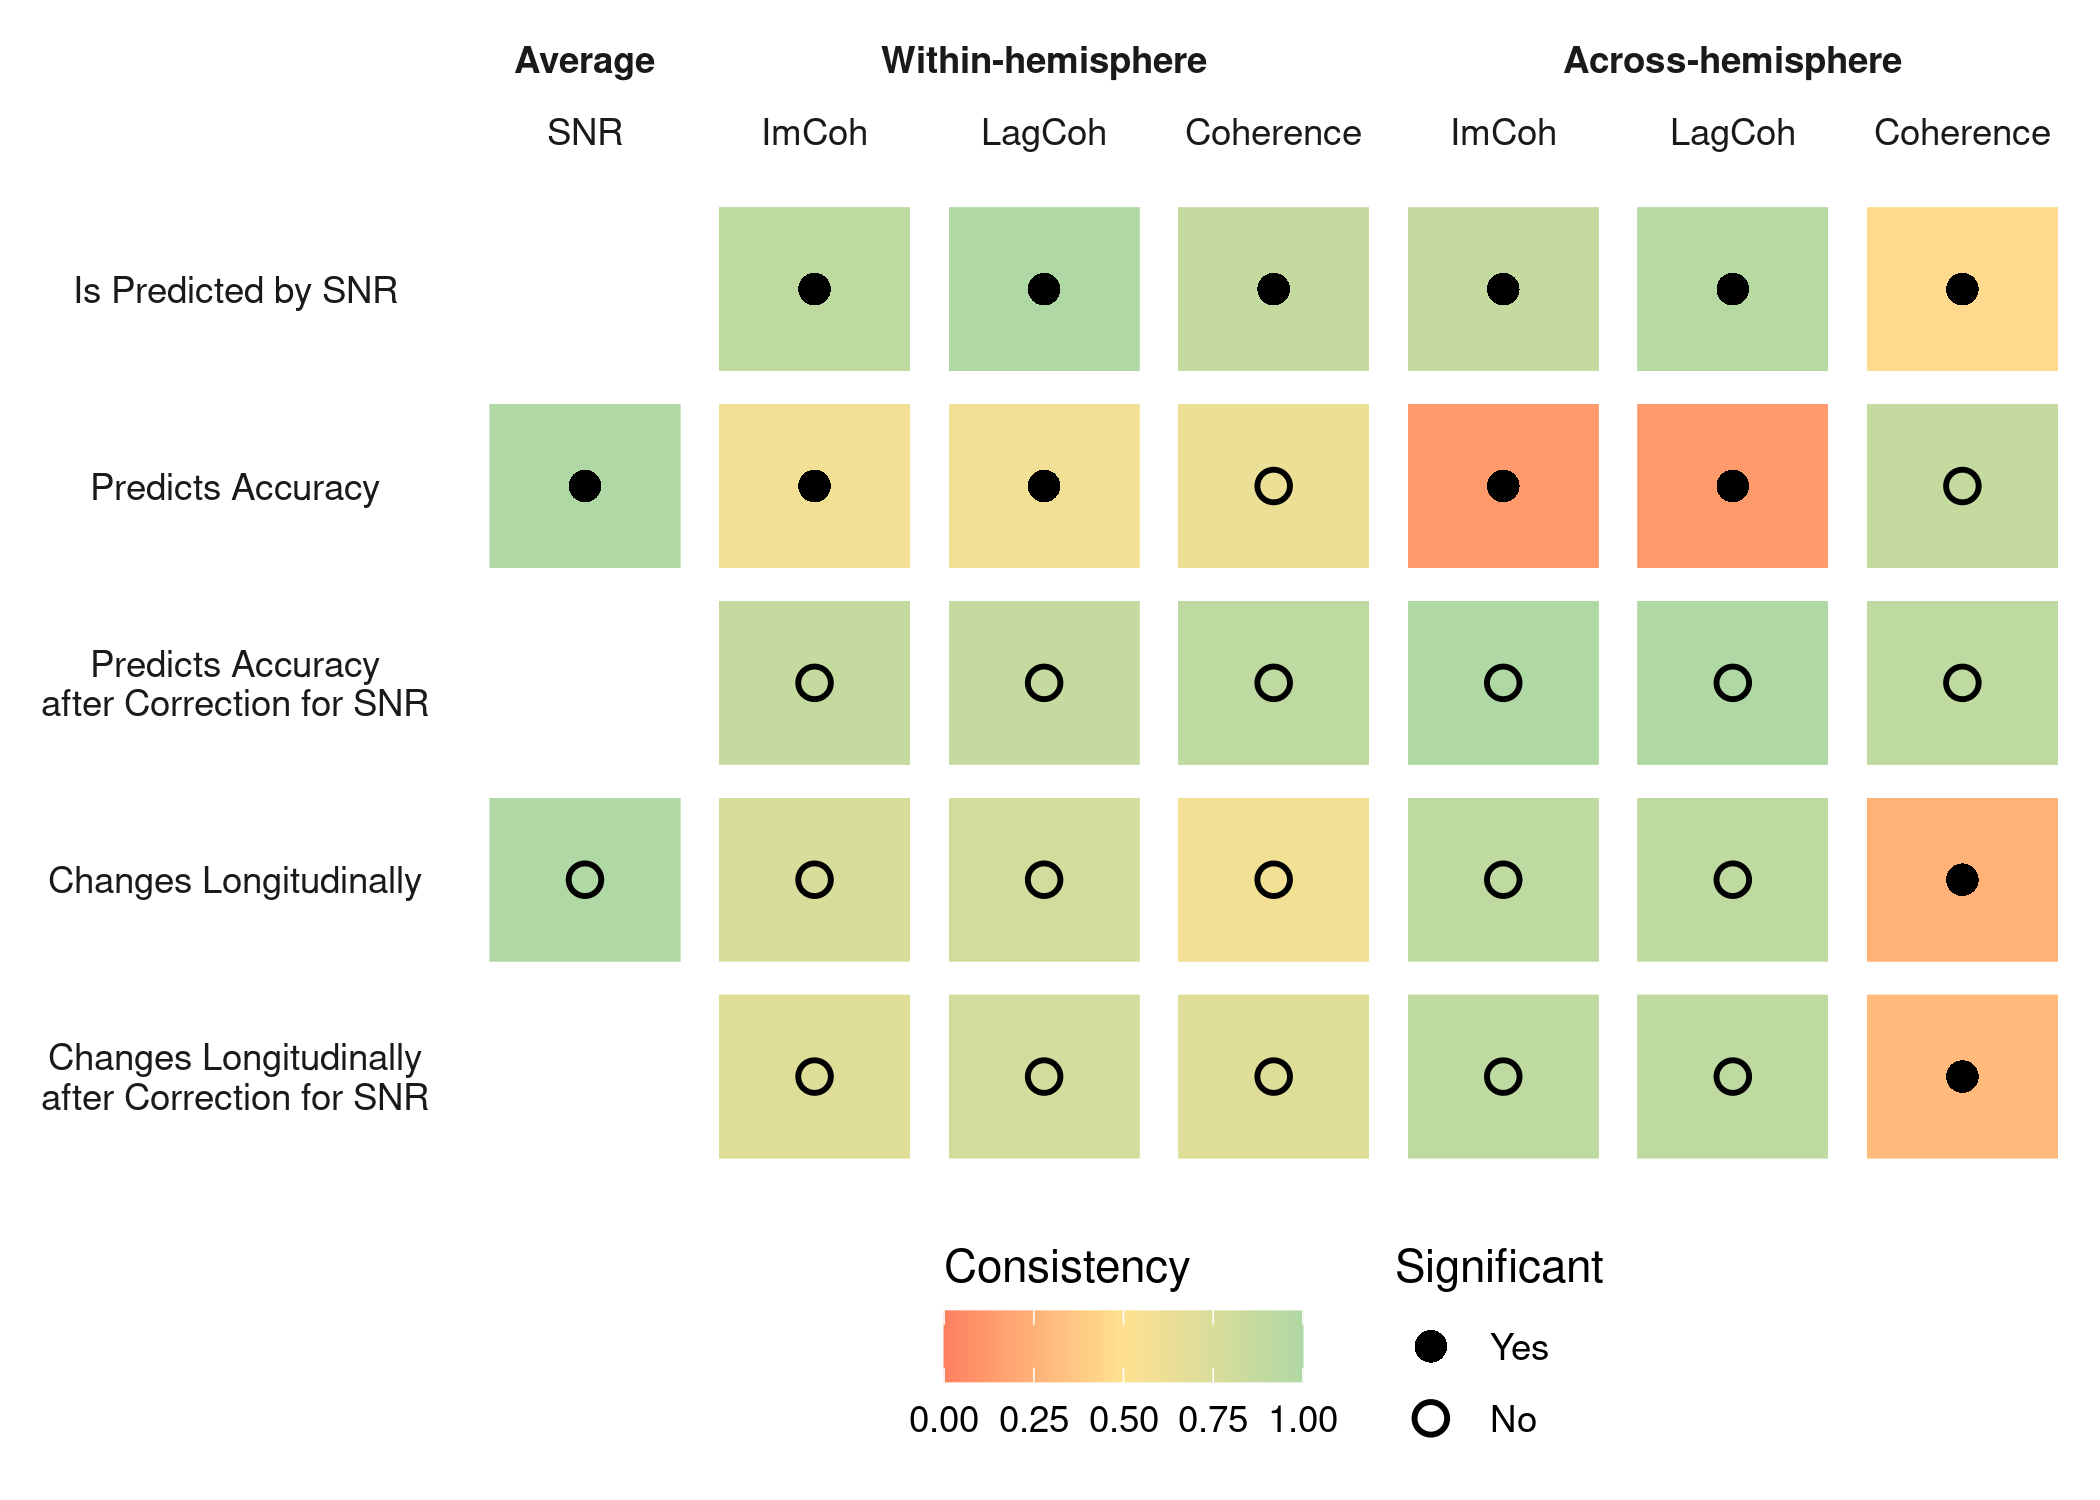
\includegraphics[width=0.9\textwidth]{fig7-multiverse-joint-analysis.png}
    \caption{Overview of the observed within-subject effects in the joint multiverse analysis. Bonferroni correction for multiple ($m=\numComparisons$) comparisons was applied to account for several phase synchronization measures. Color codes the number of pipelines that led to the same statistical result as the joint analysis.}
    \label{fig:multiverse_joint_analysis}
\end{figure}

\subsection{The selection of processing methods affected the estimated values of SNR and PS}

Effects of processing methods on the estimated values of SNR and PS were assessed with a linear mixed model. Processing steps were modeled as fixed effects, and we investigated whether the selection of the pipeline systematically affected the estimated values of SNR and PS. Table \ref{tab:pipeline_effects_summary} contains the estimated t-values for all predictors, and significant effects are highlighted in bold. Stars indicate that the effects remained significant after the correction for multiple comparisons.

\medskip

First, we observed that the values of SNR were higher when LCMV was used for inverse modeling as compared to eLORETA (Fig. \ref{fig:pipeline_effects_highlights}A), while other processing steps did not have a significant effect on SNR. We investigated the increase in SNR in more detail since the quality of the source reconstruction with LCMV depends on the SNR \citep{LCMV_VanVeen1997}, and SNR played an important role in the previous analyses. For this purpose, we compared values of SNR within pairs of pipelines, which differed only in the method for inverse modeling. As shown in Fig. \ref{supp-fig:snr_lcmv_eloreta}, the difference in the estimated SNR between the pipelines that include LCMV and eLORETA was positive and most pronounced for low values of SNR. For higher values for SNR, the difference either vanished or became negative. 

\medskip

PS measures were affected by the selection of methods for all processing steps. When the 3SVD method was used for the extraction of ROI time series as compared to 1SVD, coherence decreased (Fig. \ref{fig:pipeline_effects_highlights}C,F), while ImCoh increased. Filtering in a narrow frequency band significantly decreased all PS measures apart from within-hemisphere coherence, and Fig. \ref{fig:pipeline_effects_highlights}B and \ref{fig:pipeline_effects_highlights}E illustrate this effect for within- and across-hemisphere ImCoh, respectively. Additionally, for within-hemisphere phase synchronization, AVG-F and anatomical definitions of ROIs led to an increase in ImCoh and LagCoh as well as a decrease in coherence compared to 1SVD and task-based definitions of ROIs, respectively. Finally, LCMV led to smaller values of ImCoh and LagCoh than eLORETA (Fig. \ref{fig:pipeline_effects_highlights}D).

\begin{table}[htbp]
    \small
    \centering
    \resizebox{\linewidth}{!}{\pipelineEffectsSummary}
    \caption{Summary of the observed effects (t-values) of different processing methods on the estimated values of SNR and phase synchronization. Significant effects are highlighted in bold, and stars indicate that the effects remained significant after Bonferroni correction for multiple ($m = \numComparisons$) comparisons. Columns correspond to different processing steps, and a positive t-value for $Y | X$ denotes that SNR or PS was higher when $Y$ was used compared to $X$. X $|$ SNR denotes that a correction for SNR was applied. WH and AH stand for within- and across-hemisphere, respectively.}
    \label{tab:pipeline_effects_summary}
\end{table}

\begin{figure}[htbp]
    \centering
    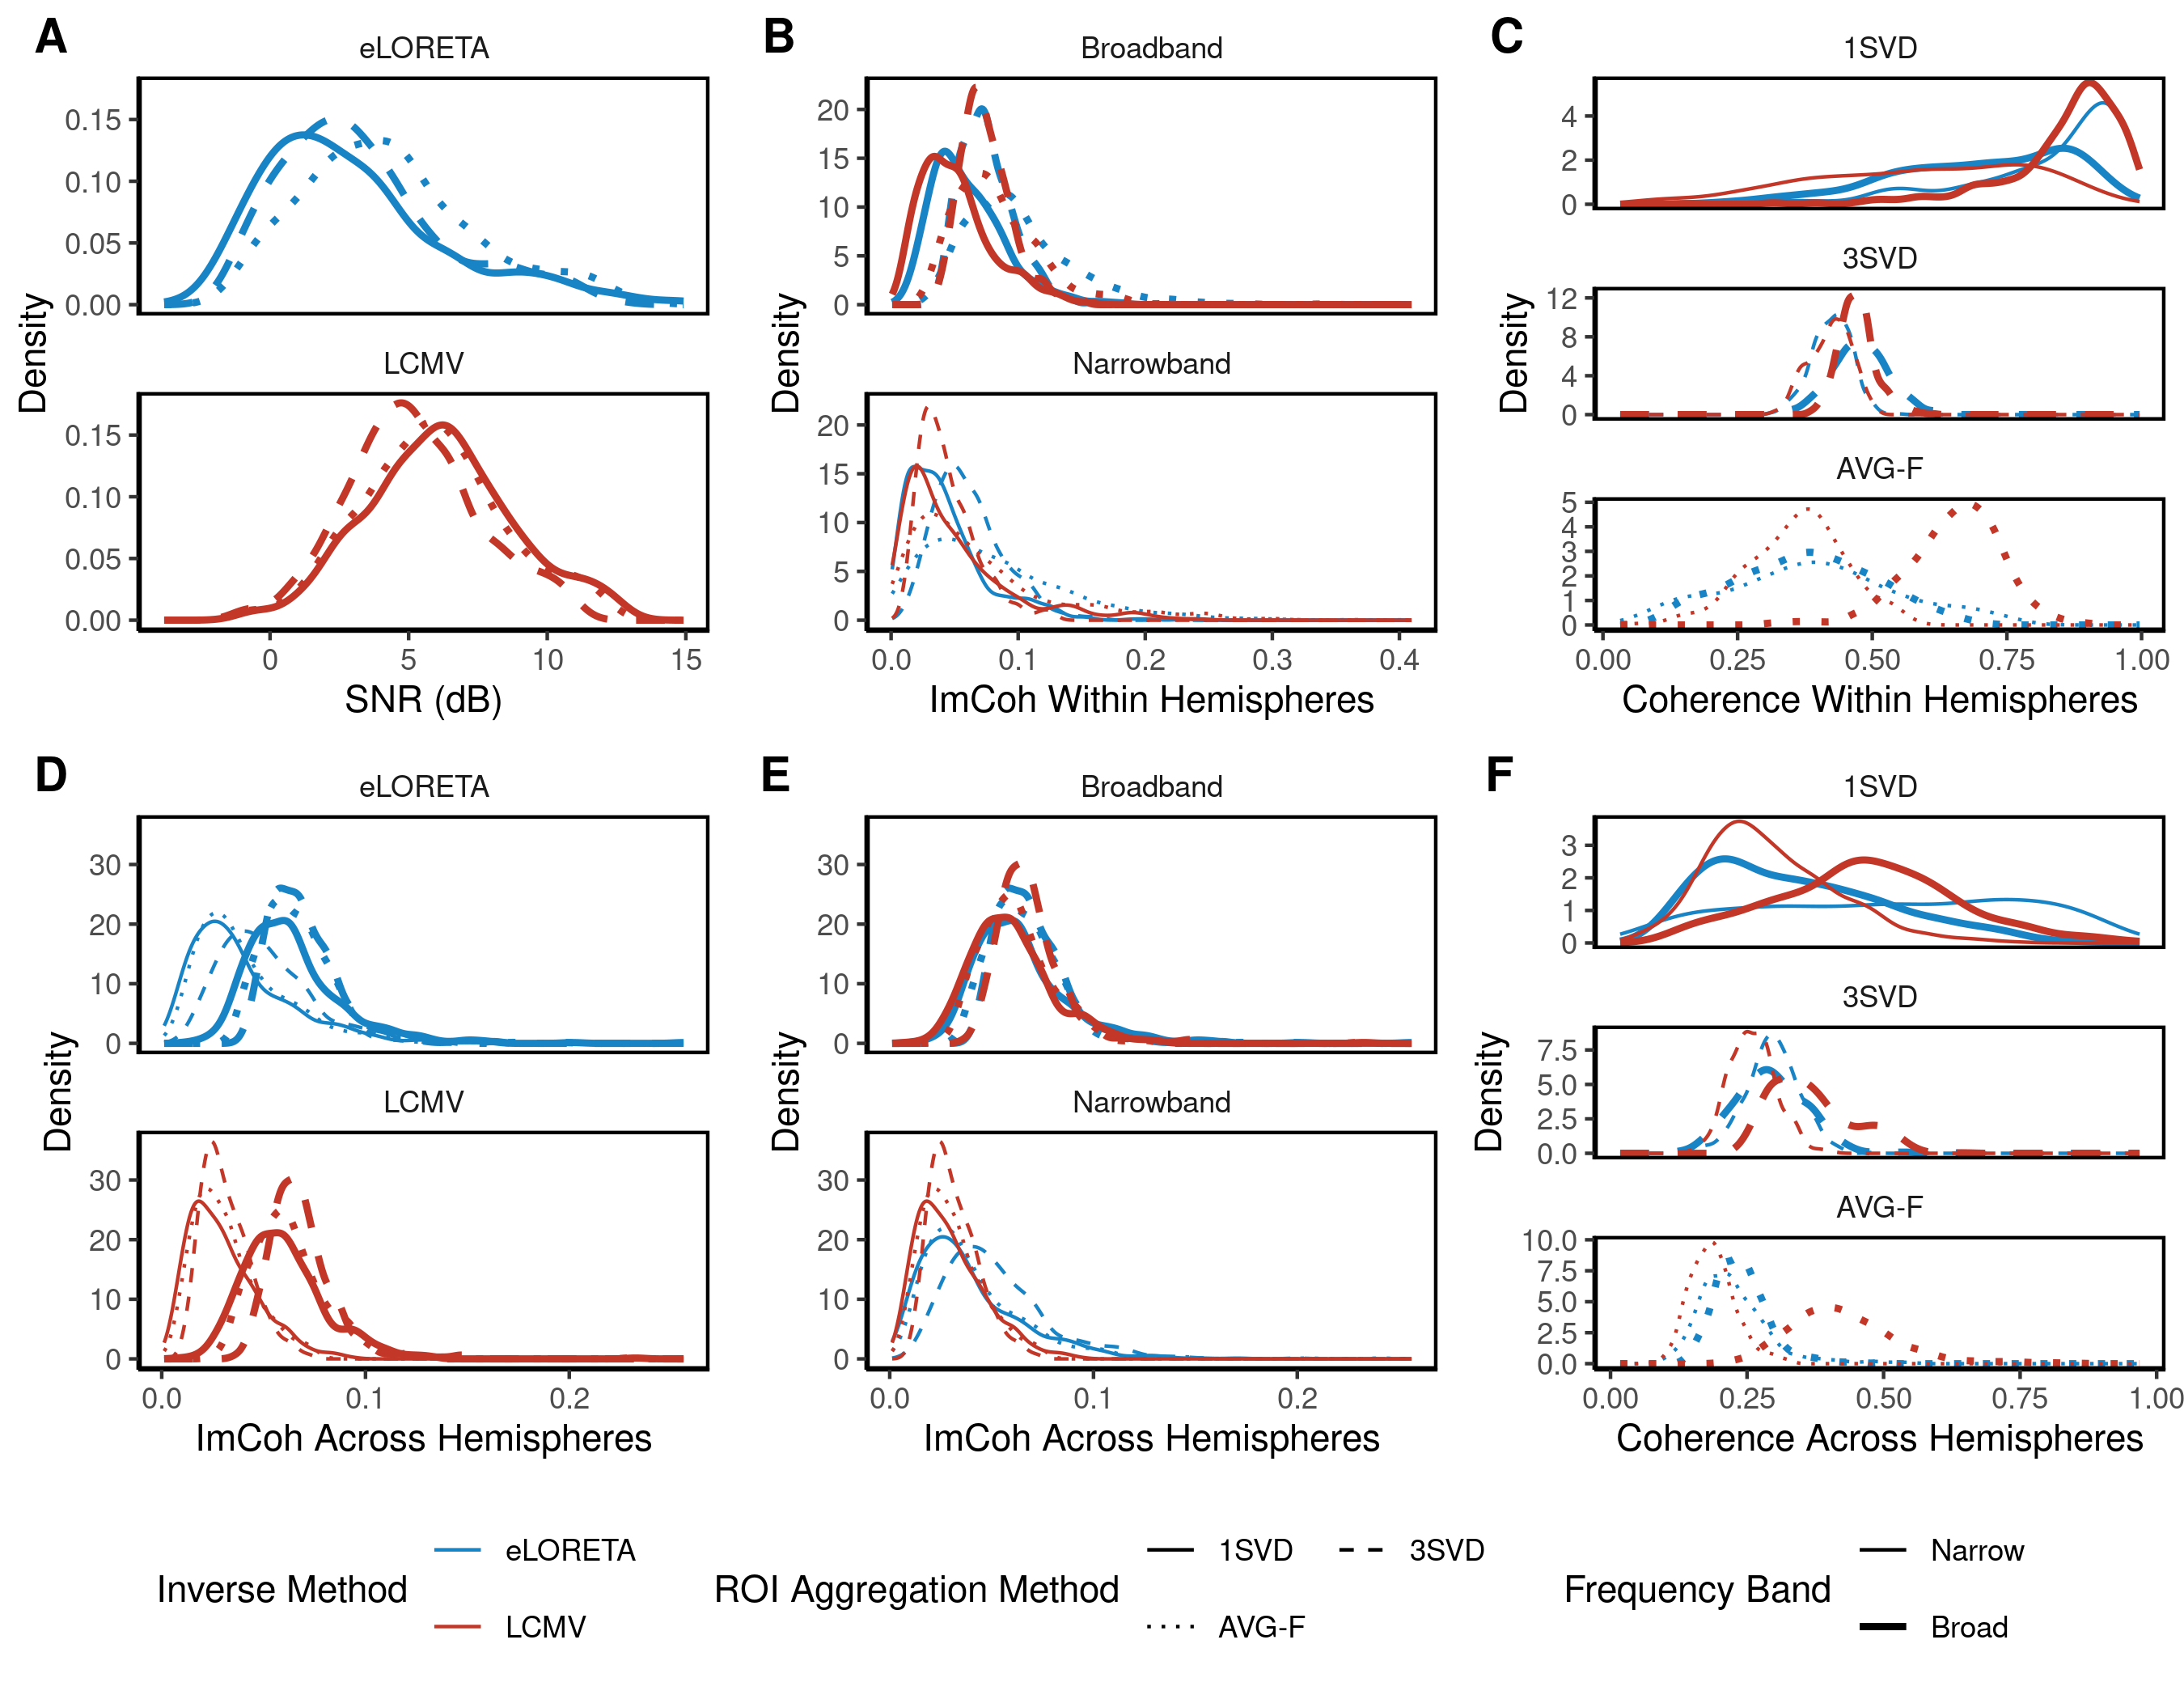
\includegraphics[width=\textwidth]{fig8-pipeline-effects-highlights.png}
    \caption{Selection of the processing methods affected estimated values of SNR and phase synchronization as indicated by shifts in the empirical probability density functions. Only pipelines with anatomical definitions of ROIs (No Mask) are displayed. (A) SNR was higher when LCMV was used as compared to eLORETA. (B) Filtering in a narrow frequency band led to smaller values of ImCoh within hemispheres. (C) Method for extraction of ROI time series affected values of within-hemisphere coherence. (D) LCMV led to smaller values of across-hemisphere ImCoh compared to eLORETA. (E) Same as B, but for ImCoh across hemispheres. (F) Same as C, but for across-hemisphere coherence.}
    \label{fig:pipeline_effects_highlights}
\end{figure}
